\documentclass[twocolumn, 10pt, conference]{ieeetran}
\usepackage[noadjust]{cite}
\usepackage{graphicx}

\title{Can Post Processing Filters Mitigate the risks of Photosensitive Epileptic Seizures?}
\author{Emiljano Bajram Kurbiba}

\begin{document}

\maketitle

\section{Authors Note}
Prior to delving into my research, it is vital to mention to the reader of this document that while an EEG test is one of the best ways to read and register brain activity, the concept of a seizure is highly dependent on the circumstances of which the patient was under. Readings can also be misinterpreted, giving false positives to a lot of diagnoses. In fact, in his book regarding epileptic research, 'The Epilepsies: Seizures, Syndromes, and Management' \cite{panayiotopoulos2005epilepsies} C.P Panayiotopoulous argues that the misinterpretation is also due to the lack of readings that occur whilst a patient is undergoing a seizure. So, whilst reading this, please understand that this study is made from findings that were done by licensed professionals and not by me.

\section{Introduction}
Epilepsy affects 1 in 100 people in the UK, \cite{EpilepsyFacts} 3\% of those being Photosensitive Epileptics. Photosensitive Epilepsy (PSE) is a type of epilepsy that is triggered by visual stimuli. This form of epilepsy has been investigated extensively by licensed professionals within the epileptic research field, it can be argued that not much is being done in the games industry to not only tackle it, but to also pander to their epileptic customers. This report explores and challenges why that is. Along with understanding why the game development community is not doing much in this specific area this project will also to reduce the risks of seizures through modern visual technology that games developers use. Post processing is one of the first visual elements a player is presented with when gaming. Post processing is a filter system added to the game-play, as the name suggests it applies the effects after game contents initial render, this means the system can work on the content as one whole image instead of different objects in game. This system makes use of such visual technology like Motion Blur, HDR, Bloom, PhysX and more. Motion Blur is used in racing games to simulate breaking, slowing down, making sharp turns and more. HDR \& Bloom is used to simulate the contrast adjustment among other purposes much like the human eye does. With such technology available this project could be possible; the objective is to collect triggering data that can be controlled and apply that data to a filter and test to see if it has reduced risks of seizure in video game.

\section{Current Status of Photosensitive Epilepsy in the Video Games Industry}
Before any action is taken it is vital to understand why not much is being done in this medium. The Video Game industry has tackled Photosensitive Epilepsy in such a way that is not adequate enough for epileptics. However, there are some examples of the industry challenging this (for example, console vendors take this seriously; Sony displays this message on their PlayStations specifically 3 \& 4):
\textbf{“Photosensitive epilepsy, if you have a history of epilepsy or seizure, consult a doctor before use, certain patterns may trigger seizures with no prior history. Before using this product, carefully read the instruction manual”} Further guides are produced by Vendors such as Sony (PlayStation) \cite{PSHealth}, Microsoft (Xbox) \cite{MicrosoftHealth} \& Nintendo (Wii)\cite{NintendoHealth}
Some Games also show a warning before a player enters the game.
\begin{figure}[h]
	\centering
	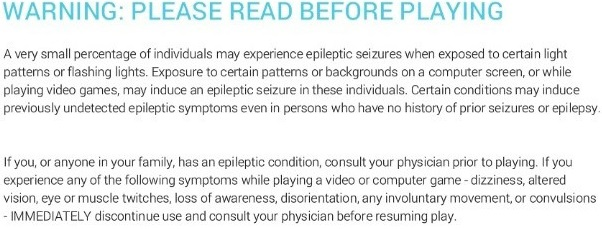
\includegraphics[width=1\linewidth]{Warning}
	\caption{}
	\label{fig:warning}
\end{figure}
\\This message in itself is indicative of the steps game developers take to separate themselves from fault, if an epileptic seizure were to occur in one of their customers they are legally exempt from fault because of this message. It should also be noted that a customer with PSE would have to buy the product before this information is available to them. Yao-Chung Chuang wrote a report titled “Massively Multiplayer Online Role-Playing Game-Induced Seizures: A Neglected Health Problem in Internet Addiction” in it he argues that that internet addiction is a growing psychological problem but PSE responses are being ignored, he observed 10 patients while playing Massively Multiplayer Online Role-Playing Games (MMORPGs) and most of the results came back with generalised tonic-clonic activity. He went on to note that “an epileptic seizure warning did not always appear on the websites of MMORPGs and instructions for the software.” \cite{Chuang}
While nothing is being done practically it is unfair to say that the industry ignores this problem completely, much like the film industry the games industry does react accordingly if incidents occur, this will be explored in the next section.

\subsection{History of Photosensitive Epilepsy in Media and Cases of Study}
One of the most famous cases of photosensitive epilepsy is the incident that occurred on December 16th 1997, where the parents of 93 children reported seizures to local emergency services because their children were watching an animated television series called “Pocket Monsters” (a Pokémon themed television show). The seizures were arguably triggered due to a scene that alternated between red and blue colours at 12Hz for 4 seconds. In a detailed report by Hiroyuki Takada et al it was contended that of the types of seizures the children had, 37 patients experienced Grand Mal/Generalized seizures. More reports were made to emergency services that day, however this report details documented ones.
When a player experiences a seizure or rather epileptic symptoms, it is not uncommon that developers in companies would respond almost instantly. In 2017, Riot Games (the publisher of the popular MOBA game League of Legends) received reports of people experiencing discomfort originating from the animations of log-in screen. Riot almost immediately responded with: they apologized, took down \& replaced the image, announced the fix\cite{Kudos}. 

\subsection{Specific Visual Guidelines}
Professors Arnold Wilkins \textit{et al} wrote a paper titled 'Characterising the patterned images that precipitate seizures and optimizing guidelines to prevent them'. They noted that developers in the Video games industry should follow the same guidelines as the International Telecoms Union:
1. Frequency. Flashes with a frequency greater than 3Hz are prohibited. 
2. Opposing changes in luminance. Flashes greater than or equal to 20cd/m2 is prohibited.
3. Area of flashes. Flashes greater in area than one-quarter of the screen are prohibited. 
4. Colour. Flashing very bright red imagery is not allowed
\cite{wilkins2005characterizing} This guideline implies that content should be designed around these rules and while such a method could prove effective for PSE gamers it generates limits to artists and designer’s creative ability. The implications of this could vary from simple lighting changes to redesign of a whole project. Player demographic should be considered also, why apply such dramatic design guidelines when only a small number of players will benefit from? It is these types of questions that may dismay developers from challenging such an issue.

\section{Understanding Epilepsy}
This section will be dedicated to understanding the disability, this is because further in the report cases of seizures in video games will be studied. Epilepsy is a group of neurological diseases characterized by recurrent seizures. Seizures happen as a result of a sudden surge of the brains electrical activities. Seizure types are not bound to any kind of epilepsy, each can cause a different type of seizure. We can first begin by exploring different types of seizures.

\subsection{Partial Onset}
This category of seizures is due to a specific part of the brain that is affected by the electrical activity.
\begin{itemize}
	\item \textbf{Simple Partial Seizure}: The affected area of the brain causes changes in that specific area, these could be exhibited as changes in vision, speech, emotion, sensation or any other motor activity without losing consciousness.
	\item \textbf{Complex Partial Seizure}: While like simple partial seizures this type is a result of a much larger affected area of the brain changes being that it causes confusion to the individual \& they experience a change in awareness.
\end{itemize}

\subsection{Primary Generalized}
Unlike Partial Onset this category is due to the entire brain being affected simultaneously.
\begin{itemize}
	\item \textbf{Generalized Tonic-Clonic or Grand Mal Seizure (GMS)}: Loss of consciousness, falling \& uncontrollable movements. 
	\item \textbf{Absence}: Brief loss of consciousness and staring.
	\item \textbf{Myoclonic}: This type of seizure causes the individual to experience brief uncontrollable muscle jerks.
	\item \textbf{Tonic}: Sudden uncontrollable movement jerks and/or extension of limbs along with the tension of the muscles.
\end{itemize}
\begin{figure}[h]
	\centering
	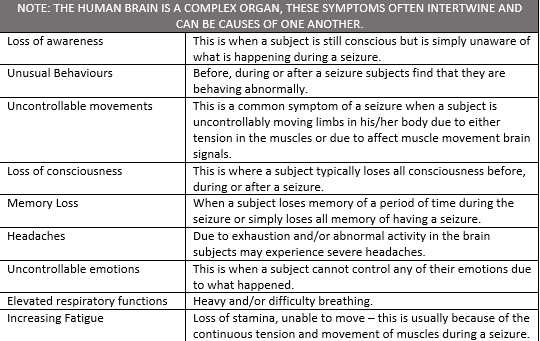
\includegraphics[width=1\linewidth]{Table}
	\caption{}
	\label{fig:table}
\end{figure}

\textbf{Loss of awareness} is when a subject is still conscious but is simply unaware of what is happening during a seizure. \textbf{Unusual Behaviours} usually occur Before, during or after a seizure subjects find that they are behaving abnormally. \textbf{Uncontrollable Movements}, this is a common symptom of a seizure when a subject is uncontrollably moving limbs in his/her body due to either tension in the muscles or due to affect muscle movement brain signals. \textbf{Memory Loss} is another symptom of a seizure, subjects usually lose memory of the seizure and maybe some time prior. After a seizure has taken place subjects may find that they experience headaches due to exhaustion and/or abnormal activity in the brain.
This information was provided by Nick Kane \textit{et al} thanks to A revised glossary of terms most commonly used by clinical electroencephalographers and updated proposal for the report format of the EEG findings. Revision 2017 \cite{kane2017revised}

\subsection{A Study on The Brain}
This section is for the reader to understand what is going on in the brain during the seizure, the figure below shows different parts of the brain and what they are responsible for.
\begin{figure}[h]
	\centering
	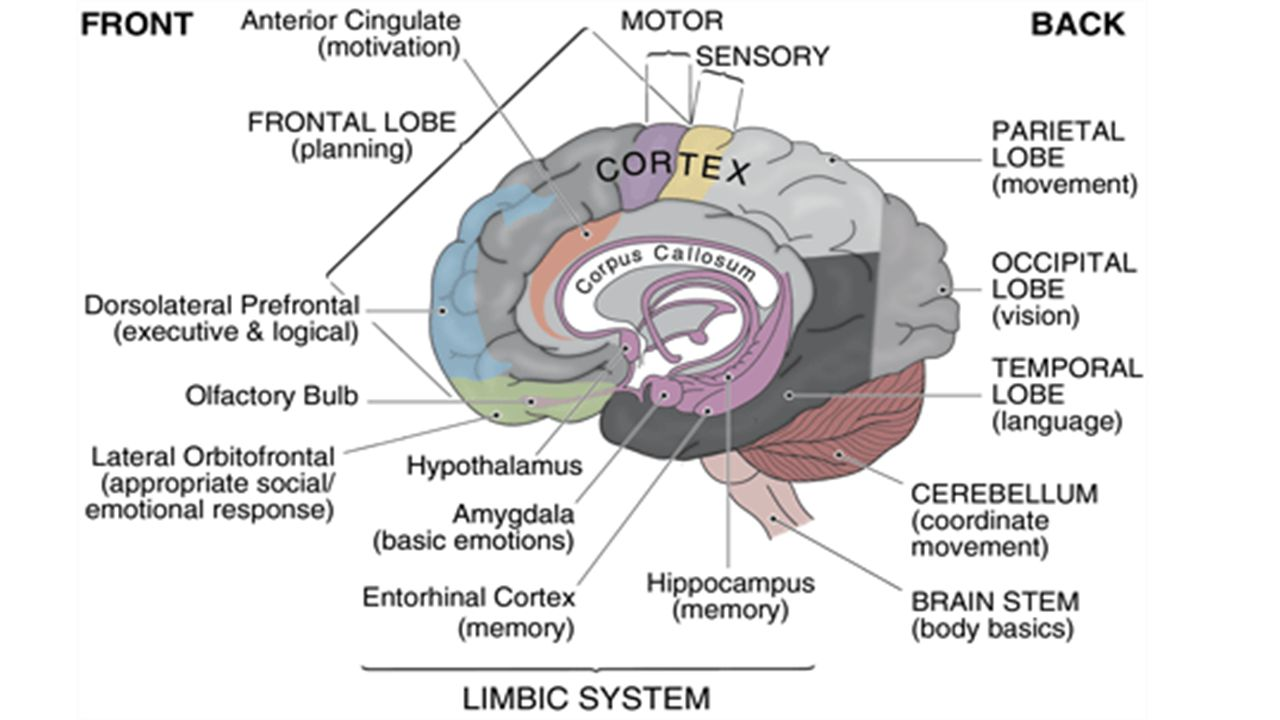
\includegraphics[width=1\linewidth]{a7c4617a0cd51b6a39119417ae3cd24e}
	\caption{}
	\label{fig:Brain Described}\cite{BrainUnderstand}
\end{figure}
Photic seizures occur when neurons in the visual cortex (occipital lobe) are over-stimulated, thus creating a large electrical current that is fired across the brain, in turn, giving the recipient the above figure 2 symptoms. Notice here since the visual cortex is located at the back of the brain, and when neurons get excited and initiate a seizure notice that the Parietal Lobe (Movement), Temporal lobe (Language) \& Cerebellum (Coordinate Movement) are at risk the most; should these areas be affected it could be the origin of some symptoms such as uncontrollable movement, uncontrollable voice \& unusual behaviours.

\subsection{Measuring Epilepsy}
The continuous recording of brain activity in a Photosensitive epilepsy patient is measured through Electro-encephalography (EEG). When neuron data is received by dendrites in the brain, it causes an electrical polarity change - and these changes are continuously recorded. A single polarity change is too small to measure, however when thousands of changes occur in one location it becomes more visible: this is called Local Field Potential (LFP).\\
This is all measured by applying caps to the user that measure different focal points of the brain, which in turn is connected to an EEG amplifier which amplifies the signal strength. The amplifier is then connected to a computer. Specific caps also measure eye and muscle movements, and this is called Electrooculogram (EOG)
\begin{figure}[h!]
	\centering
	\includegraphics[width=1\linewidth]{"Figure 3"}
	\caption{}
	\label{Figure 4:EEG Reading}
\end{figure}
\textbf{Figure 4} is what a typical EEG data stream looks like, the numbers on the left side representing points of measurement. Small passive wavelengths are typically measured as normal brainwaves while strong high-frequency waves are characterized by muscle movement. Wavelengths are typically divided into 4 main groups:
\\\\
\begin{itemize}
	\item \textbf{Delta}: delta group lies in the 1-4Hz range it’s the most passive type of reading, these wavelengths occur when we are not doing much or in deep sleep (Specifically not dreaming).
	\item \textbf{Theta}: Theta group lies in the 4-8Hz range, difficult cognitive processing such as calculating the sum of 219 times 384 is what produces this kind of wavelength.
	\item \textbf{Alpha}: Alpha group lies in the 8-12Hz range, it is responsible for measuring our senses. States such as paying attention, relaxing, concentrating and so on. 
	\item \textbf{Beta}: Beta group lies within the 12-25hz range, these wavelengths usually are readings of movements or when we are planning to move.
	\item \textbf{Gamma}: Gamma range lies within 25+Hz. There is not a specific reason or cause for this range but popular theories state that these wavelengths are responsible for perception and consciousness. \cite{kane2017revised}
\end{itemize}
Emiliana Pellouchoud et al conducted an experiment to identify if there were differences between juvenile subjects with epilepsy and normal control subjects when they are actively playing a game. They concluded that all patients had similar results however interestingly enough all the patients were engaged in the game and this is easily read without being there due to their wavelength readings. Increases from 6-7 Theta, 9-12 Alpha \& 10-13 beta were shown meaning all patients were challenged, relaxed and tended to move during gameplay.\cite{pellouchoud1999mental} This data also proves that video games can provide photomyoclonic, or photoconvulsive responses within epileptic patients.

\subsection{Wavelength Behaviour in Photosensitive Epilepsy}
Commonly researchers use wavelength behaviour to determine activity in Photosensitive epilepsy. While this data alone can be used to measure normal brain processing, it is what is associated with or what the patient is doing that diagnoses PSE activity.
\begin{itemize}
	\item \textbf{Sharp wave} - Transient, clearly distinguishable from background activity, with pointed peak at conventional paper speeds and a duration of 70-200 milliseconds (ms)
	\item \textbf{Spike} - Same as sharp wave, but with duration of 20 to less than 70 ms
	\item \textbf{Sharp-and-slow-wave complex} - Pattern consisting of a sharp followed by a slow wave (clas-sically the slow wave being of higher amplitude than the sharp)
	\item \textbf{Spike-and-slow-wave complex} - Pattern consisting of a spike followed by a slow wave (clas-sically the slow wave being of higher amplitude than the spike)
	\item \textbf{Multiple spike-and-slow-wave complex} - Same as spike-and-slow-wave complex, but with 2 or more spikes associated with one or more slow waves
\end{itemize}
In a report titled ‘Game-Related Seizures Presenting with Two Types of Clinical features’ by Yao-Chung Chuang \cite{chuang2006game} \textit{et al}, a test was conducted to see what type of seizures could be caused by video games. They tested 22 people with a history of photosensitive epilepsy, aged 13-40, with a computer-generated version of the Japanese board game, Mah-Jong, and other various game type. Interestingly, results proved positive, indicating a change in PSE activity. A detailed table showed some patients experiencing sharp waves whilst others remained with normal EEG activity, signifying that while patients were linked up to EEG’s, it is possible for video games to induce or aggravate a seizure.

\section{Data Applicable to Games Development}
Considering research and guidelines obtained previously in the report (see page 2, under Specific Visual Guidelines) suggest that the biggest threats to a PSE patient would be brightness, contrast differences, red coverage and the frequency in which those variables are displayed at. All these variables are controllable through post processing volumes; however, brightness is a value that simply depends on the user’s hardware (monitor), and the lowest dynamic nit range found in monitors during research was 200-250 nits (Cd/m2). In theory, while at this range an effect can be applied to limit brightness, new-found monitor technology such as HDR and Apple iMac panels can reach a range of 500-1000 Nits (Cd/m2). While gamers are unlikely to play on such productivity intense monitors. it should not be dismissed and considered in depth. Evidently, this is why multiple iterations of post processing volumes may need to be developed.\\
Extensive research has been done on refresh rates additionally, in ‘The effect of television frame rate on EEG abnormalities in photosensitive and pattern-sensitive epilepsy.’,\cite{fylan1997effect} professor G. Harding discusses refresh rates and its effects during an EEG exam. To simplify, their results specify that the subjects that were exposed to a device displaying 100Hz – in which the chances of an epileptic response were reduced by more than half, making them less prone to a seizure. Thus, a higher refresh rate is required for reduced seizure risks. According to iiYama, one of the leading Computer Monitor manufacturers in the world, the average refresh rate for a monitor is 60Hz. However, over the past few years companies are pushing for higher refresh rates in its panels as it offers a smoother display.

\section{Proposal \& Methodology}
Utilizing the Data applicable to game development and considering research conducted by medical specialists, this project will seek to create a post-processing filter that counters high dynamic seizure inducing game content. Upon completion, the effect results/data will be recorded both visually and data will be statistically compared to perceive if the project was successful or a failure. Nevertheless, due to ethical reasons, the institution permitting this project forbids human test subjects.

\subsection{Test Environment}
A test environment is crucial for this project. A level will be created to test the post-processing effect that is why the research was conducted to find the most visually stimulating real-world environment to recreate digitally. Due to its visually stimulating signs and lights, a place called the Shinjuku District of Japan was chosen for this project. It should be noted that to further the visual stimulation a neo-Tokyo theme was added to the environment. The setting of the film ‘Akira’, or perhaps the setting in the game trailer of ‘Cyberpunk 2077’ by CD Projekt Red is a perfect example of what this project is trying to achieve visually. To verify, this scenery will attempt to induce a seizure and a program called Photosensitive Epilepsy Analysis Tool (PEAT) will be used to verify the epileptic response.

\subsection{Photosensitive Epilepsy Analysis Tool}
The primary tool to determine the results of this seizure-inducing content will be ‘Photosensitive Epilepsy Analysis Tool’, a program created by the trace research and development centre at the University of Maryland. It is a very powerful tool to detect seizure inducing content, and the developers even conducted an interview with one of the world’s leading pioneers in PSE research Dr. Graham Harding for guidance on the creation of the program. The program captures any video or window that is provided, and then analyses it frame by frame for a risk assessment. Currently, it has had four conditions pass, indicating that it is risk free. However, in order to understand this process, it is important to be aware that: Caution (Pass) will mean that it is a majority pass but still has the small possibility of failure and cause a seizure, Caution (Fail) by the majority will indicate that the content will be very likely to cause a seizure, whilst a fail will signify that it will always absolutely fail.

\subsection{Post Processing Application}
The leading objective of the application is to simply be able to play the prototype with a post-processing effect applied that proves to reduce the risk of seizure. Many iterations of the effect will be applied and with the help of source-control, each change made to the effect will be documented. With the effect applied, gameplay will be recorded and then played back to capture (through the PEAT program) for analysis. Upon analysis, the fail or success rate will be signified.

\subsection{Final Results}
After the test is run to determine the success rate of the filter the data used for development, it will then be analysed and further discussed briefly to comprehend how it impacted the game and whether or not it is viable enough to become common practice in the game development industry. The final section of the dissertation will be an answer to the question and analysis to find improvements along with self-reflection on how or what I could have done better.

\bibliographystyle{IEEEtran}
\bibliography{References}
\end{document}

